\documentclass[preview, border={0pt 0pt 2pt 2pt}]{standalone}
\usepackage{amsmath}
\usepackage{graphicx}
\usepackage{tikz, pgfplots}
\usepackage{graphicx}
\begin{document}
\begin{tikzpicture}
  \pgfplotsset{width=10cm, height=5cm}
  \begin{axis}[
    axis lines=left,
    xlabel=,
    every outer x axis line/.append style={-},
    every outer y axis line/.append style={-},    
    ylabel=Singular Value,
    ylabel near ticks,
    xmin=-0.5, xmax=5.5,
    ymin=0, ymax=1.5,
    xtick={0,...,5},
    ytick={0,0.5,...,1.5},
    xticklabels={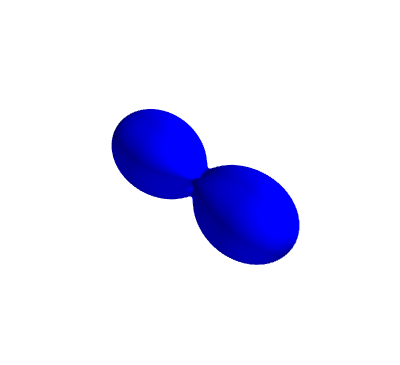
\includegraphics[scale=0.125]{sv0},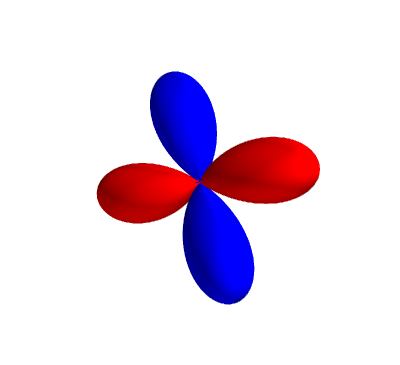
\includegraphics[scale=0.125]{sv1}, 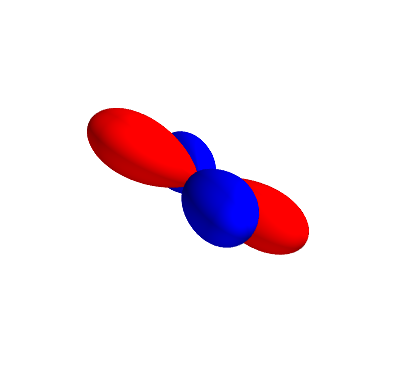
\includegraphics[scale=0.125]{sv2},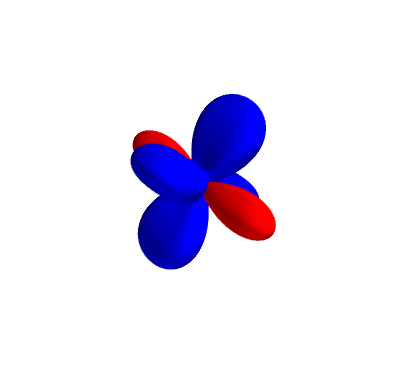
\includegraphics[scale=0.125]{sv3},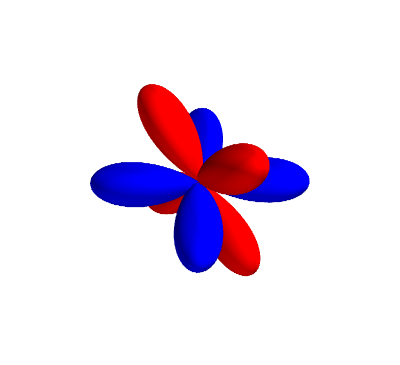
\includegraphics[scale=0.125]{sv4}, 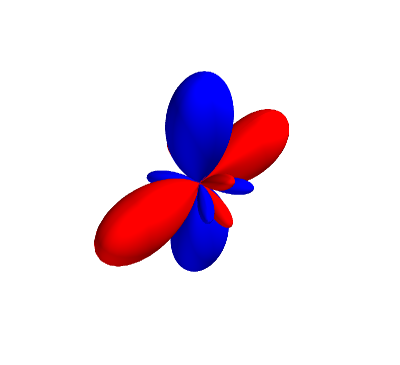
\includegraphics[scale=0.125]{sv5}},
    xticklabel style={yshift=5pt},
    ] 
    \addplot+[
    ycomb,
    black,
    mark options={black}
    ] plot coordinates
	{(0,1.36) (1,0.43) (2,0.43) (3,0.38) (4,0.22) (5,0.03)};
\end{axis}
\end{tikzpicture}
\end{document}
